
\begin{figure*}[t]
    \setlength{\resLen}{1.75in}
    %
    \centering
    \small
    \setlength{\tabcolsep}{1pt}
    \renewcommand{\arraystretch}{0}
    %
    %
    \begin{tabular}{cccc}
        % &
        \textbf{Reference} & (a) \textbf{Ours} & (b) \textbf{3DGS} & (c) \textbf{3DGRT}
        \\[3pt]
        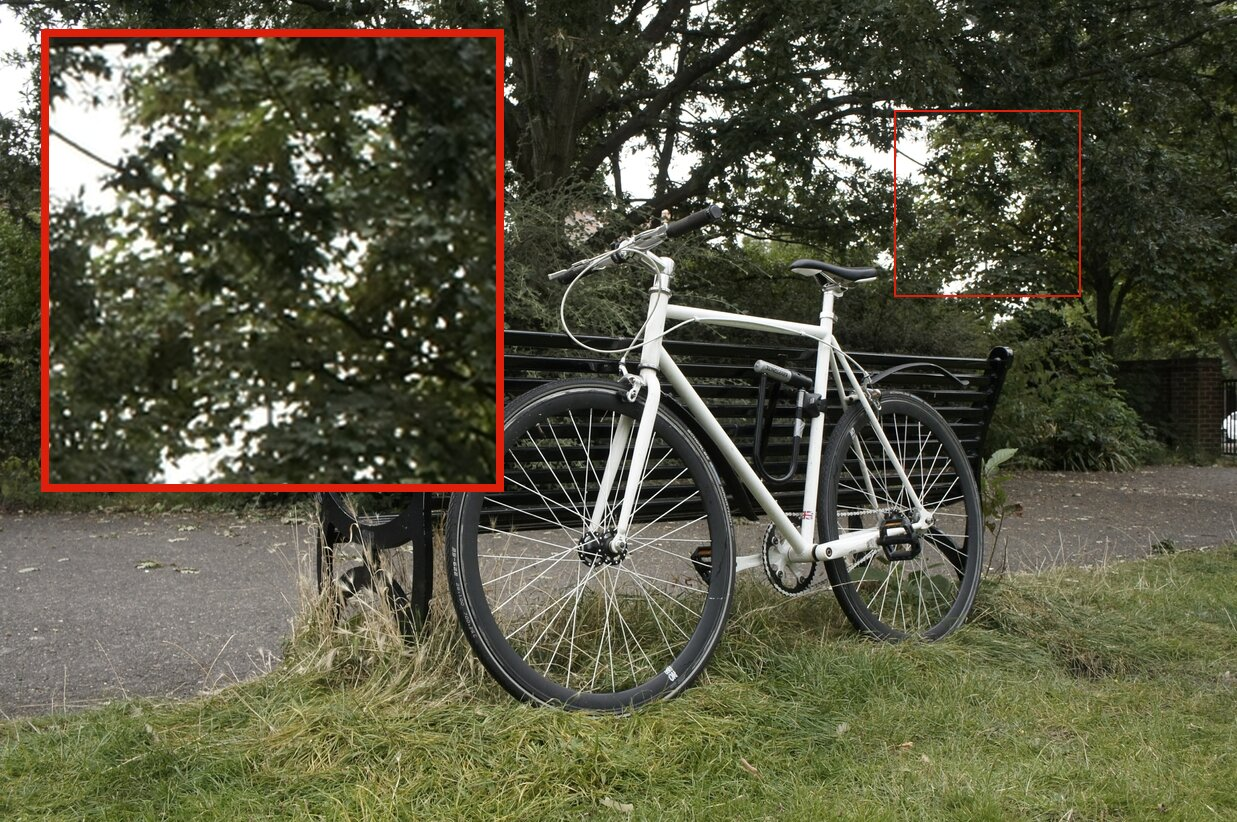
\includegraphics[width=\resLen]{images/equal-time/bicycle/reference_composite.jpg} &
        \imgwithtext{\resLen}{\contour{black}{PSNR 19.0 / SSIM 0.541}}{images/equal-time/bicycle/quasistoch_composite.jpg} &
        \imgwithtext{\resLen}{\contour{black}{PSNR 19.0 / SSIM 0.544}}{images/equal-time/bicycle/3dgs_composite.jpg} &
        \imgwithtext{\resLen}{\contour{black}{PSNR 18.2 / SSIM 0.529}}{images/equal-time/bicycle/3dgrt_composite.jpg} 
        \\[3pt]
        
\includegraphics[width=\resLen]{images/equal-time/bonsai/reference_composite.jpg} &
        \imgwithtext{\resLen}{\contour{black}{PSNR 30.5 / SSIM 0.931}}{images/equal-time/bonsai/quasistoch_composite.jpg} &
        \imgwithtext{\resLen}{\contour{black}{PSNR 31.5 / SSIM 0.942}}{images/equal-time/bonsai/3dgs_composite.jpg} &
        \imgwithtext{\resLen}{\contour{black}{PSNR 29.6 / SSIM 0.925}}{images/equal-time/bonsai/3dgrt_composite.jpg} 
        \\[3pt]
        % 
\includegraphics[width=\resLen]{images/equal-time/counter/reference_composite.jpg} &
        % 
\includegraphics[width=\resLen]{images/equal-time/counter/ours_composite.jpg} &
        % 
\includegraphics[width=\resLen]{images/equal-time/counter/3dgs_composite.jpg} &
        % 
\includegraphics[width=\resLen]{images/equal-time/counter/3dgrt_composite.jpg} 
        % \\[3pt]
        
\includegraphics[width=\resLen]{images/equal-time/room/reference_composite.jpg} &
        \imgwithtext{\resLen}{\contour{black}{PSNR 29.8 / SSIM 0.918}}{images/equal-time/room/quasistoch_composite.jpg} &
        \imgwithtext{\resLen}{\contour{black}{PSNR 28.8 / SSIM 0.908}}{images/equal-time/room/3dgs_composite.jpg} &
        \imgwithtext{\resLen}{\contour{black}{PSNR 27.4 / SSIM 0.880}}{images/equal-time/room/3dgrt_composite.jpg} 
        % \\[3pt]
        % 
\includegraphics[width=\resLen]{images/equal-time/stump/reference_composite.jpg} &
        % 
\includegraphics[width=\resLen]{images/equal-time/stump/ours_composite.jpg} &
        % 
\includegraphics[width=\resLen]{images/equal-time/stump/3dgs_composite.jpg} &
        % 
\includegraphics[width=\resLen]{images/equal-time/stump/3dgrt_composite.jpg} 

    \end{tabular}
    %
    \caption{\textbf{Equal-time comparison} between our method and baselines. All methods run for the same wall-clock time. Our method produces comparable visual quality to 3DGS and outperforms 3DGRT.
    }
    \label{fig:nvs_figures}
\end{figure*}


\begin{figure*}[t]
    \setlength{\resLen}{1.75in}
    %
    \centering
    \small
    \setlength{\tabcolsep}{1pt}
    \renewcommand{\arraystretch}{0}
    %
    %
    \begin{tabular}{cccc}
        % &
        \textbf{Reference} & (a) \textbf{Ours} & (b) \textbf{RNG} & (c) \textbf{GS$^3$}
        \\[3pt]
        % 
\includegraphics[width=\resLen]{images/relightable/lego/reference_composite.jpg} &
        % \imgwithtext{\resLen}{PSNR 30.4 / SSIM 0.949}{images/relightable/lego/ours_composite.jpg} &
        % \imgwithtext{\resLen}{PSNR 26.7 / SSIM 0.924}{images/relightable/lego/RNG_composite.jpg} &
        % \imgwithtext{\resLen}{PSNR 26.6 / SSIM 0.923}{images/relightable/lego/GS3_composite.jpg}
        % \\[2pt]
        
\includegraphics[width=\resLen]{images/relightable/basket/reference_composite.jpg} &
        \imgwithtext{\resLen}{\contour{black}{PSNR 28.0 / SSIM 0.956}}{images/relightable/basket/ours_composite.jpg} &
        \imgwithtext{\resLen}{\contour{black}{PSNR 20.0 / SSIM 0.853}}{images/relightable/basket/RNG_composite.jpg} &
        \imgwithtext{\resLen}{\contour{black}{PSNR 23.2 / SSIM 0.936}}{images/relightable/basket/GS3_composite.jpg}
        \\[2pt]
        % 
\includegraphics[width=\resLen]{images/relightable/furball/reference_composite.jpg} &
        % \imgwithtext{\resLen}{PSNR 33.7 / SSIM 0.949}{images/relightable/furball/ours_composite.jpg} &
        % \imgwithtext{\resLen}{PSNR 27.8 / SSIM 0.926}{images/relightable/furball/RNG_composite.jpg} &
        % \imgwithtext{\resLen}{PSNR 26.4 / SSIM 0.931}{images/relightable/furball/GS3_composite.jpg}
        % \\[2pt]
        
\includegraphics[width=\resLen]{images/relightable/hotdog/reference_composite.jpg} &
        \imgwithtext{\resLen}{\contour{black}{PSNR 31.9 / SSIM 0.955}}{images/relightable/hotdog/ours_composite.jpg} &
        \imgwithtext{\resLen}{\contour{black}{PSNR 30.4 / SSIM 0.960}}{images/relightable/hotdog/RNG_composite.jpg} &
        \imgwithtext{\resLen}{\contour{black}{PSNR 25.4 / SSIM 0.949}}{images/relightable/hotdog/GS3_composite.jpg}
    \end{tabular}
    %
    \caption{Reconstruction quality of our method and baselines on the relightable benchmark. Our method produces significantly better geometry, especially shadow quality.
    }
    \label{fig:relightable_figures}
\end{figure*}

\begin{figure*}[t]
    \setlength{\resLen}{1.2in}
    %
    \centering
    \small
    \addtolength{\tabcolsep}{-6.5pt}
    %
    %
    \begin{tabular}{cccccc}
        % &
        (a1) \textbf{Ours, original} & (b1) \textbf{Reference} & (c1) \textbf{Ours, relit} & (a2) \textbf{Ours, original} & (b2) \textbf{Reference} & (c2) \textbf{Ours, relit}
        \\
        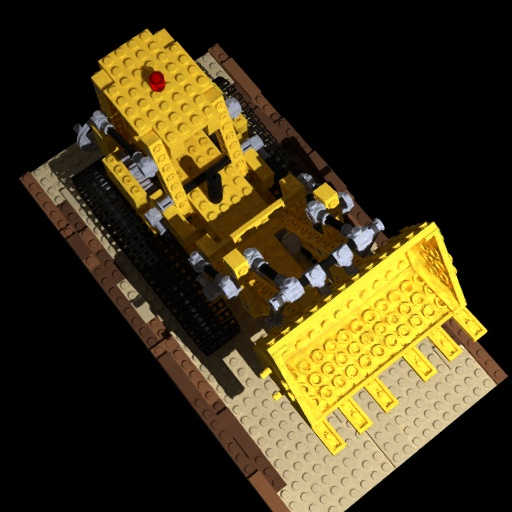
\includegraphics[width=\resLen]{images/relightable/envmap/original_cam0.jpg} &
        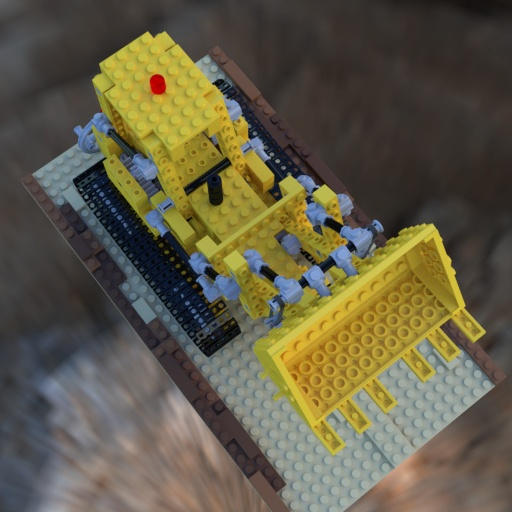
\includegraphics[width=\resLen]{images/relightable/envmap/blender_cam0_bright.jpg} &
        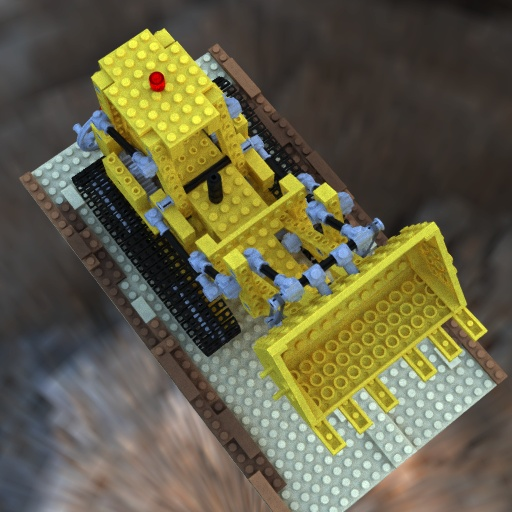
\includegraphics[width=\resLen]{images/relightable/envmap/ours_cam0_bright.jpg} &
        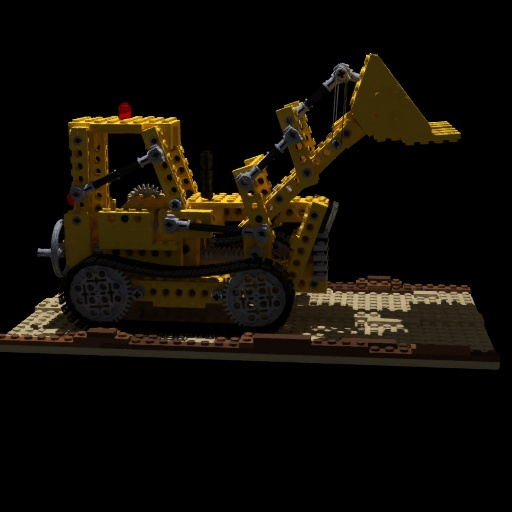
\includegraphics[width=\resLen]{images/relightable/envmap/original_cam1.jpg} &
        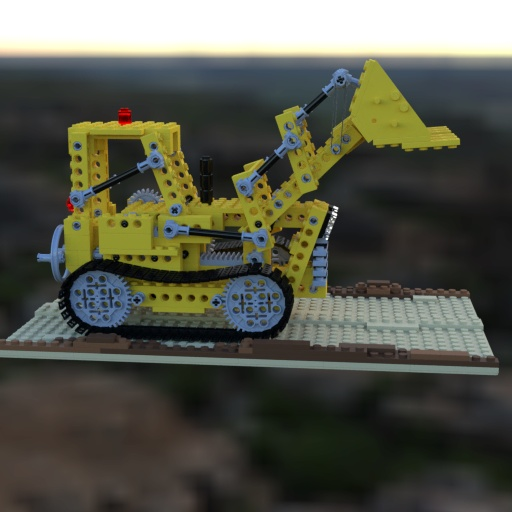
\includegraphics[width=\resLen]{images/relightable/envmap/blender_cam1_bright.jpg} &
        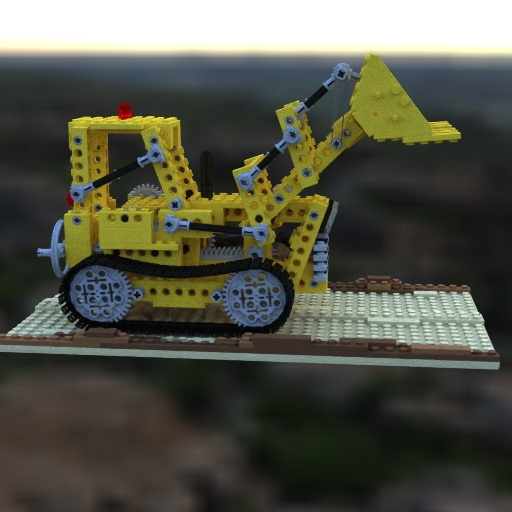
\includegraphics[width=\resLen]{images/relightable/envmap/ours_cam1_bright.jpg}
    \end{tabular}
    %
    \caption{
        Re-renderings of our reconstructed 3DGS objects under novel environmental illumination.
    }
    \label{fig:environment_map_relighting}
\end{figure*}
